\subsection{ICP s grupacijom točaka}

\subsubsection{Opis algoritma}
Koristi se voxelgrid\cite{pcl:voxelgrid} metoda. Radi tako da se cijeli oblak točaka podijeli na kocke zadane veličine te se tada unutar te kocke filtriraju točke na temelju njihove centroide. U jednome od očitanja iz primjera A se vroj točaka s 35222 smanjio na 1548 što značajno ubrzava ICP algoritam. Ovaj algoritam zapravo aproksimira skup točaka samo jednom točkom. U primjeru \ref{coderef:voxel_grouping} se vidi da je parametar visine, širine i duljine kocke uvijek jednak i iznosi 1 centimetar što znači da će se oblak točaka podijeliti na kocke veličine 1 centimetar. Performanse toga algoritma kao i točnost reprezentacije originalnog oblaka ovise o tom parametru kao i gustoći točaka.


\subsubsection{Izvorni kod algoritma}
Kod je vrlo sličan kao i u prethodnome algoritmu samo što sada imamo jedan korak više prije obrade oblaka ICP algoritmom. Doajemo linije \ref{lineref:voxel1} i \ref{lineref:voxel2}. Pozivamo metodu \ref{coderef:voxel_method}. Unutar nje se inicijalizira objekt tipa \mintinline{text}{VoxelGrid<PT>}. Kao parametre prima oblak točaka i veličinu područja na koje će podijeliti oblak točaka.

\begin{listing}[H]
  \begin{minted}[frame=lines, linenos]{text}
void downsample_using_voxel_grid(
  PointCloudType::Ptr& cloud,
  float width, float height, float length,
  PointCloudType::Ptr& downsampled
 ) {
  VoxelGrid<PT> vg;
  vg.setInputCloud(cloud);
  vg.setLeafSize(width, height, length);
  vg.filter(*downsampled);
}
  \end{minted}
  \caption{Metoda za grupaciju točaka}
  \label{coderef:voxel_method}
\end{listing}

\begin{listing}[H]
  \begin{minted}[frame=lines, linenos, escapeinside=!!]{text}
void process_files(vector<path> paths, ICP icp) {
 for (int i = 0; i < paths.size() - 1; i++) {
  if (i == 0) {
   load_point_cloud(paths.at(i).string(), *cloud_ref);
  }
  load_point_cloud(paths.at(i + 1).string(), *cloud_target);

  string first = paths.at(i).stem().string(); 
  string second = paths.at(i + 1).stem().string();

  if (i == 0) {
   downsample_using_voxel_grid(
     cloud_ref, 1.0f, cloud_ref_filtered !\label{lineref:voxel1}!
   );
  }
  downsample_using_voxel_grid(
    cloud_target, 1.0f, cloud_target_filtered !\label{lineref:voxel2}!
  );

  icp.setInputCloud(cloud_ref_filtered);
  icp.setInputTarget(cloud_target_filtered);
  icp.align(*cloud_reg);

  if (icp.hasConverged()) {
   save_matrix(icp, first, second);
  }
  *cloud_ref = *cloud_target;
 }
}
  \end{minted}
  \caption{ICP grupacija točaka - obrada oblaka}
  \label{coderef:voxel_grouping}
\end{listing}
\pagebreak
\subsubsection{Rezultat algoritma}
Kao i za prethodni algoritam rezultati su dani u tablici \ref{res:ref_est_table_vox}.

\begin{table}[H]
  \centering
  \begin{tabular}{ |p{3cm}| |p{3cm}|p{3cm}| }
    \hline
    Rezultati& Primjer A& PrimjerB\\
    \hline
    Duljina [m]& 664.451& 452.433\\
    AMx [m]& 1.676& 0.236\\
    AMy [m]& 0.671& 0.534\\
    AMz [m]& 0.021& 0.006\\
    AMr [rad]& 9.256E-4& 2.570E-4\\
    AMp [rad]& 7.189E-4& 2.061E-4\\
    AMy [rad]& 0.345& 0.003\\
    \hline
    MSEx [$m^2$]& 8.466& 0.170\\
    MSEy [$m^2$]& 2.214& 0.944\\
    MSEz [$m^2$]& 9.736E-4& 1.008E-4\\
    MSEr [$rad^2$]& 8.974E-6& 1.884E-6\\
    MSEp [$rad^2$]& 3.967E-6& 4.944E-7\\
    MSEy [$rad^2$]& 1.981E-4& 1.997E-4\\
    \hline
  \end{tabular}
  \caption{Usporedbe referentnih i estimiranih podataka}
  \label{res:ref_est_table_vox}
\end{table}
\pagebreak

\subsubsection{Evaluacija rezultata za primjer A}
\begin{figure}[H]
  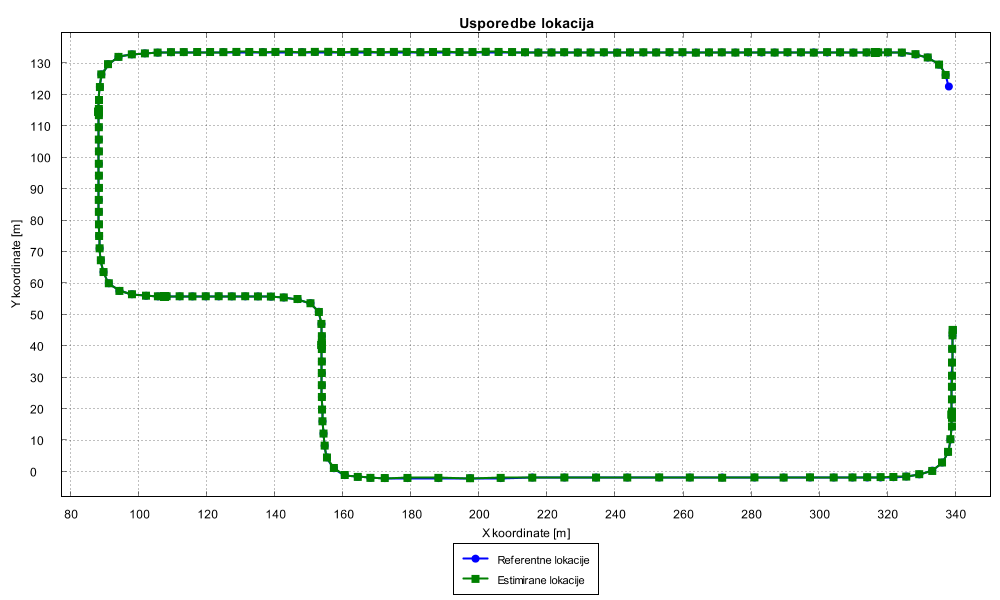
\includegraphics[scale=0.4]{images/voxel/pr3/usporedba_lokacija.png}
  \caption{Graf lokacije vozila}
  \label{eval:a2p3_lokacija}
\end{figure}
\begin{figure}[H]
  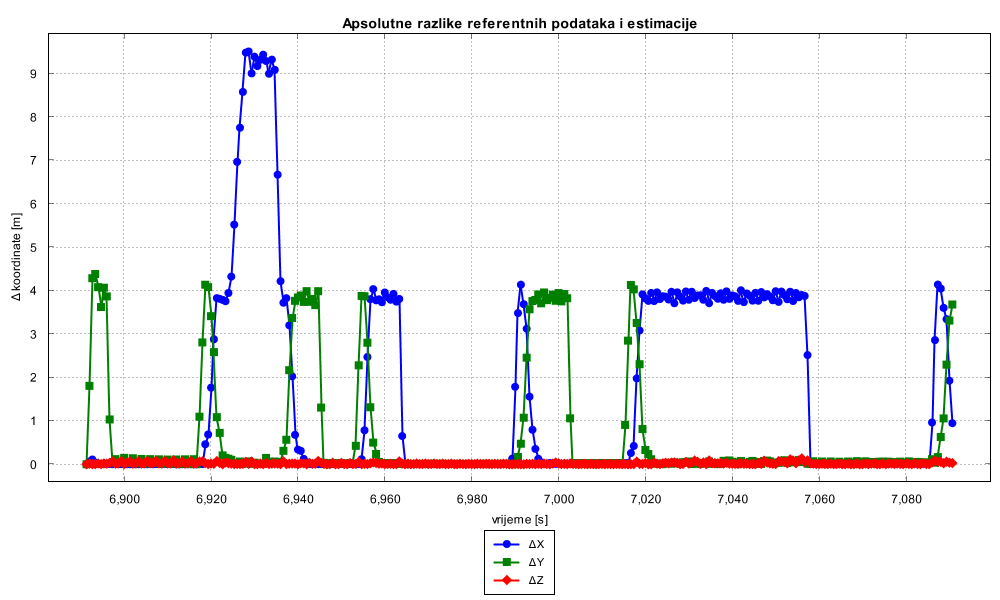
\includegraphics[scale=0.4]{images/voxel/pr3/apsolutne_razlike_koordinata.png}
  \caption{Apsolutne razlike koordinata}
  \label{eval:a2p3_koord_razlike}
\end{figure}
\begin{figure}[H]
  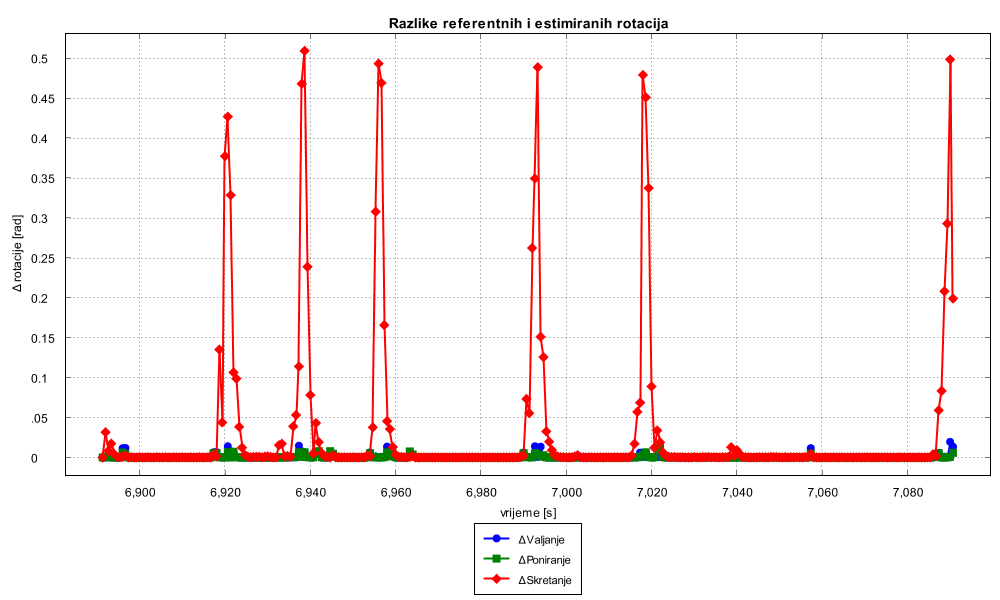
\includegraphics[scale=0.4]{images/voxel/pr3/rotacije_razlike.png}
  \caption{Apsolutne razlike rotacija}
  \label{eval:a2p3_rot_razlike}
\end{figure}
\begin{figure}[H]
  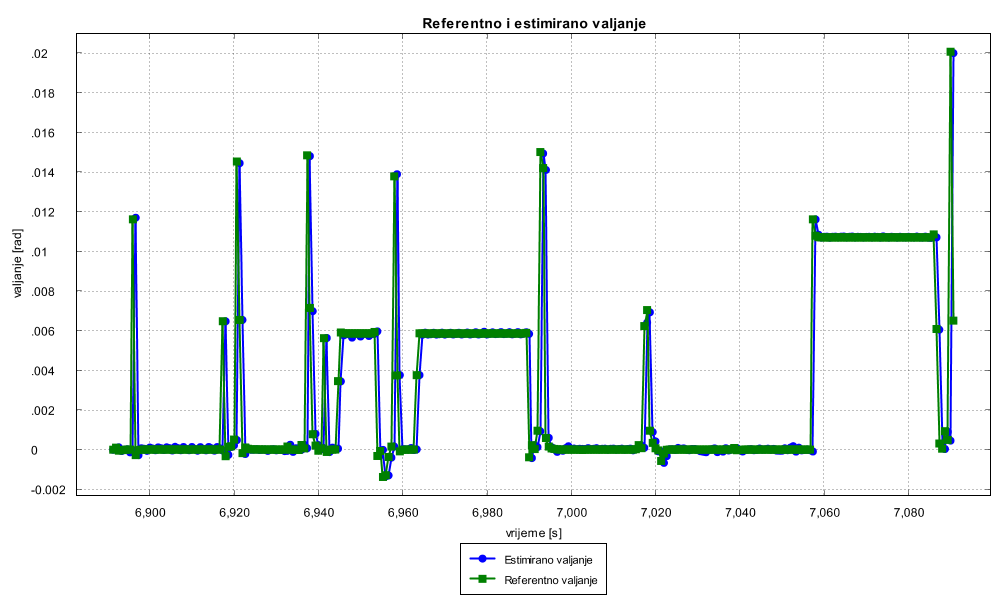
\includegraphics[scale=0.4]{images/voxel/pr3/referentno_estimirano_valjanje.png}
  \caption{Usporedba referentnog i estimiranog valjanja}
  \label{eval:a2p3_rot_roll}
\end{figure}
\begin{figure}[H]
  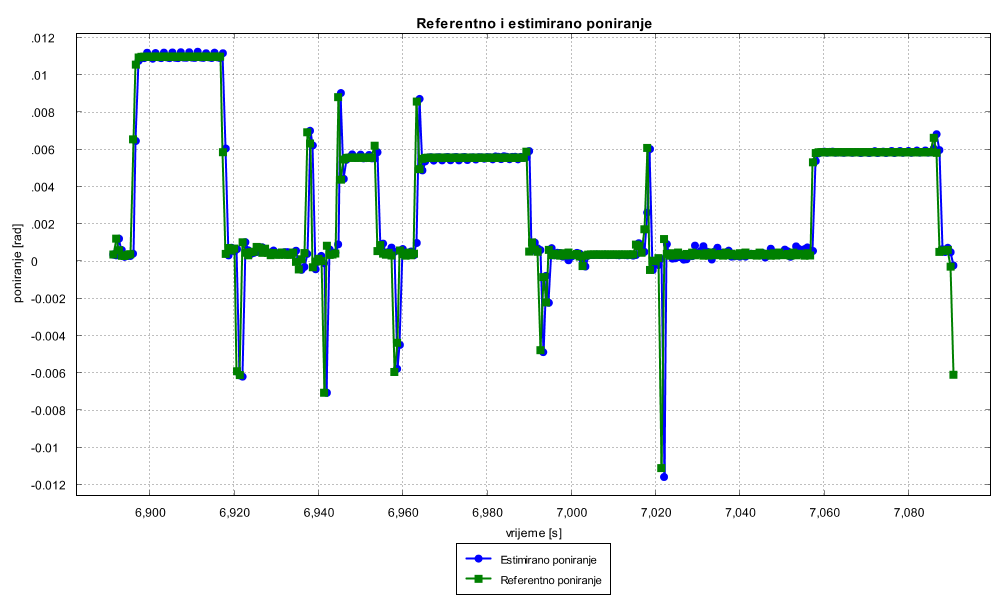
\includegraphics[scale=0.4]{images/voxel/pr3/referentno_estimirano_poniranje.png}
  \caption{Usporedba referentnog i estimiranog poniranja}
  \label{eval:a2p3_rot_pitch}
\end{figure}
\begin{figure}[H]
  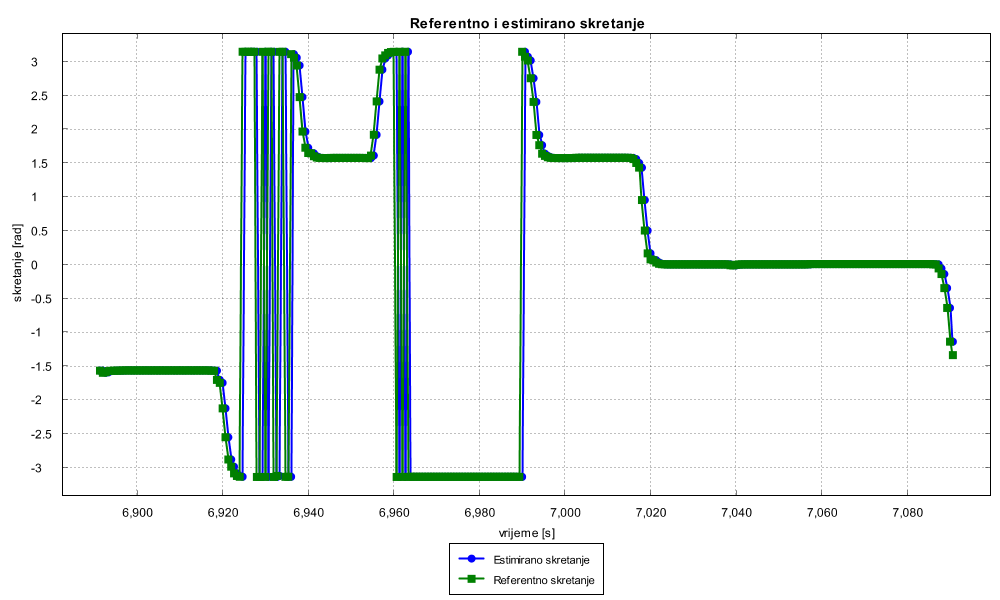
\includegraphics[scale=0.4]{images/voxel/pr3/referentno_estimirano_skretanje.png}
  \caption{Usporedba referentnog i estimiranog skretanja}
  \label{eval:a2p3_rot_yaw}
\end{figure}


\subsubsection{Evaluacija rezultata za primjer B}
\begin{figure}[H]
  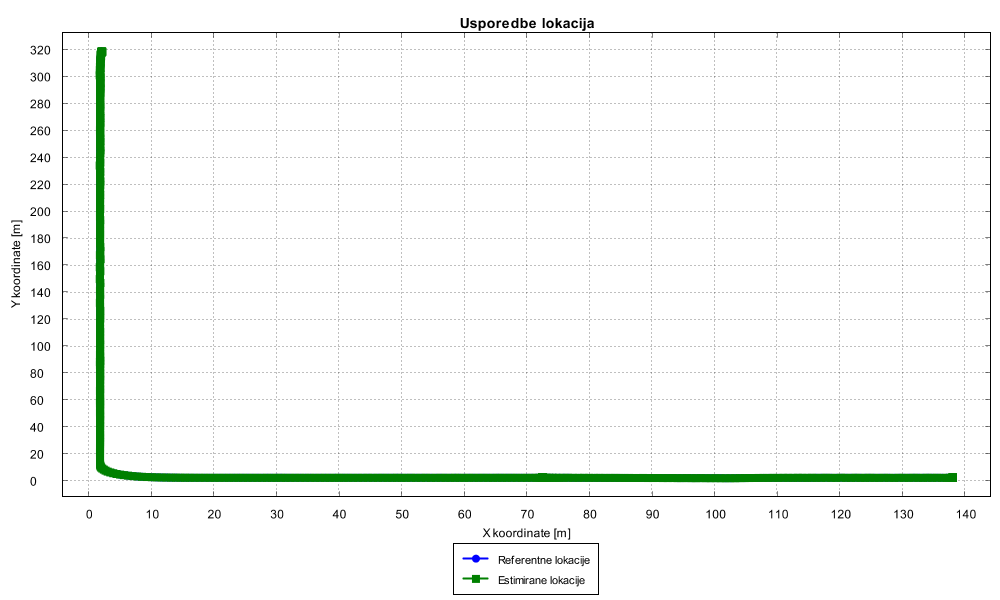
\includegraphics[scale=0.4]{images/voxel/pr4/usporedba_lokacija.png}
  \caption{Graf lokacije vozila}
  \label{eval:a2p4_lokacija}
\end{figure}
\begin{figure}[H]
  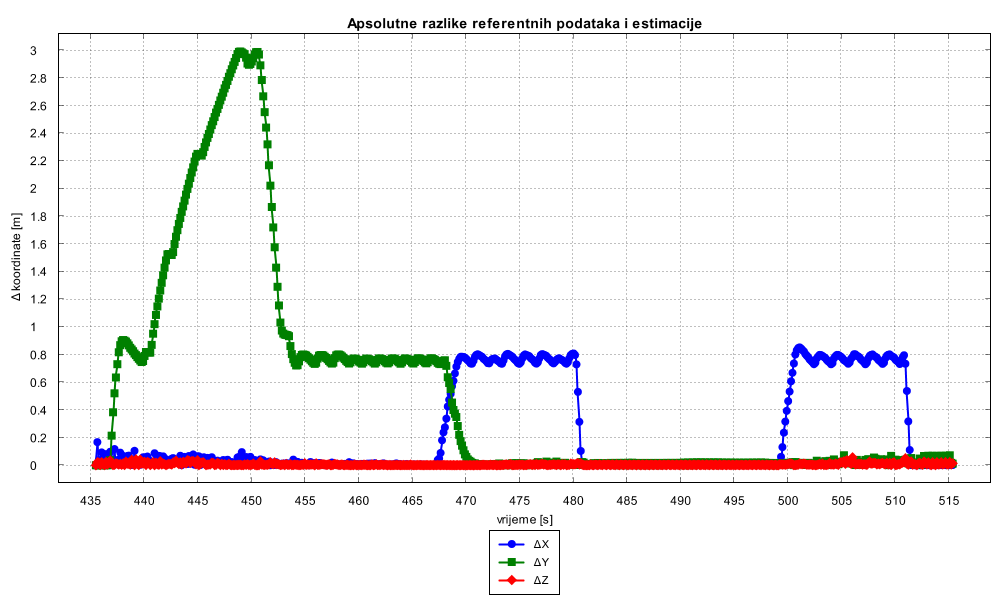
\includegraphics[scale=0.4]{images/voxel/pr4/apsolutne_razlike_koordinata.png}
  \caption{Apsolutne razlike koordinata}
  \label{eval:a2p4_koord_razlike}
\end{figure}
\begin{figure}[H]
  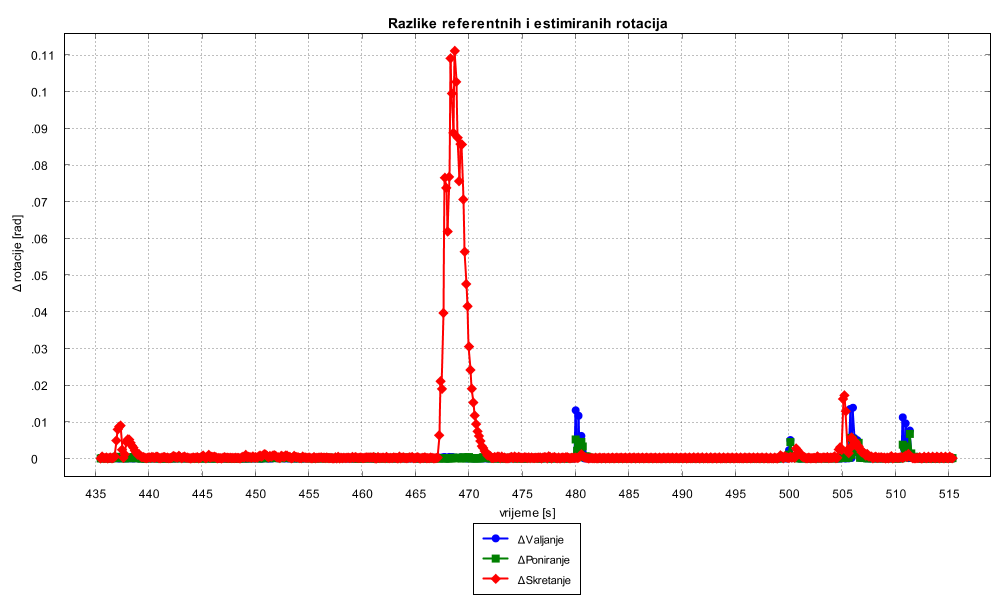
\includegraphics[scale=0.4]{images/voxel/pr4/rotacije_razlike.png}
  \caption{Apsolutne razlike rotacija}
  \label{eval:a2p4_rot_razlike}
\end{figure}
\begin{figure}[H]
  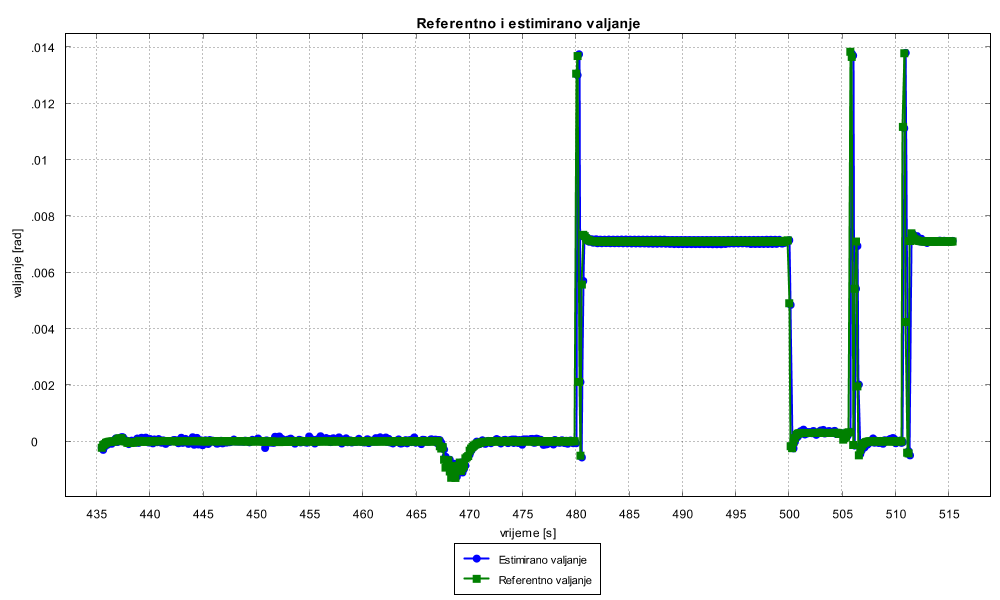
\includegraphics[scale=0.4]{images/voxel/pr4/referentno_estimirano_valjanje.png}
  \caption{Usporedba referentnog i estimiranog valjanja}
  \label{eval:a2p4_rot_roll}
\end{figure}
\begin{figure}[H]
  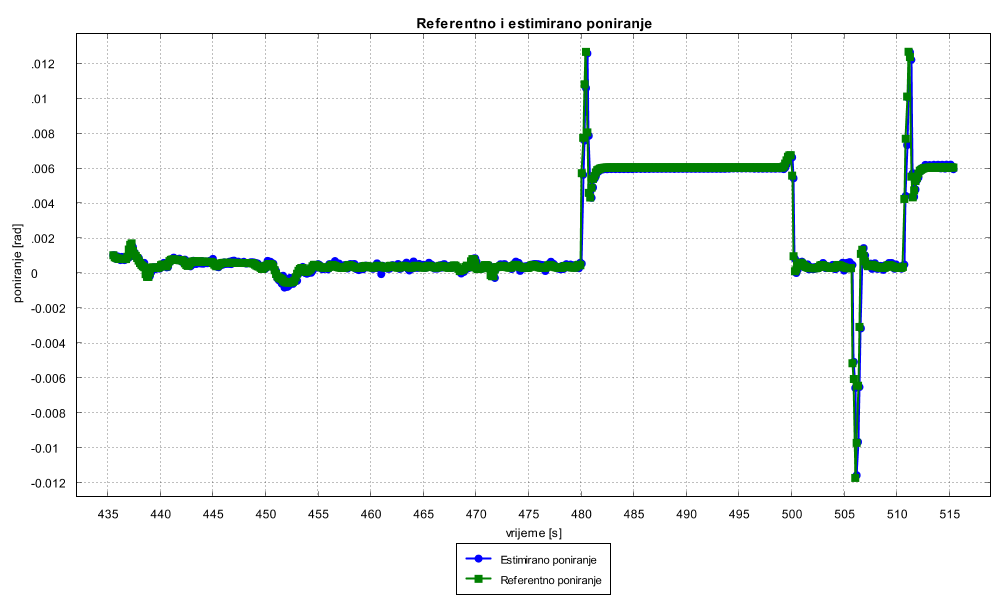
\includegraphics[scale=0.4]{images/voxel/pr4/referentno_estimirano_poniranje.png}
  \caption{Usporedba referentnog i estimiranog poniranja}
  \label{eval:a2p4_rot_pitch}
\end{figure}
\begin{figure}[H]
  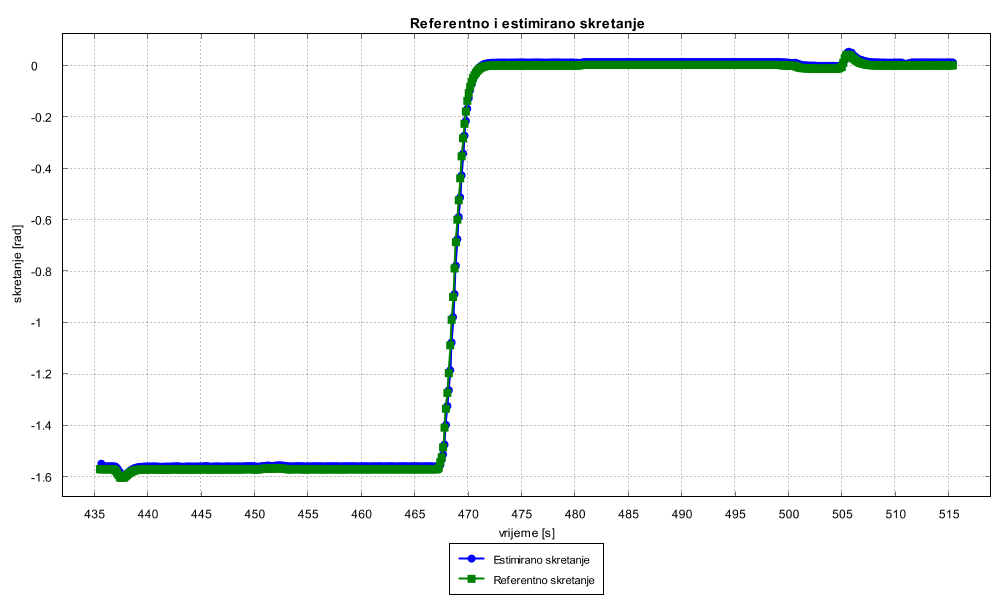
\includegraphics[scale=0.4]{images/algo1/primjer4/referentno_estimirano_skretanje.png}
  \caption{Usporedba referentnog i estimiranog skretanja}
  \label{eval:a2p4_rot_yaw}
\end{figure}
\pagebreak